%%%%%%%%%%%%%%%%% REVISÃO BIBLIOGRÁFICA %%%%%%%%%%%%%%%%%
\chapter{A demografia e o estudo da fecundidade masculina}

Este capítulo fará uma revisão de alguns dos principais estudos que analisam o padrão da FM, elencando alguns dos principais tópicos, dificuldades, especificidades e suas diferenças com relação à fecundidade feminina, no mundo e no Brasil. Serão expostos as principais bases e métodos utilizados para o cálculo das taxas de fecundidade masculinas. 

%%%%%%%%% O QUE É FECUNDIDADE MASCULINA %%%%%%%%%%


A fecundidade é um tema de grande relevância na demografia. Possui papel fundamental no estudo do ritmo do crescimento populacional, sendo uma das três componentes principais utilizadas no cálculo de projeções populacionais. É também a base de teorias demográficas que estudam padrões e mudanças na composição por grupos de idade da população e seus determinantes, como a transição demográfica \cite{FOZ2021metodos} e a transição da fecundidade \cite{mason1997explaining}.

No entanto, as formas de realizar a mensuração e análise da fecundidade são marcadas pela predominância da abordagem baseada apenas na fecundidade feminina, tanto nos indicadores produzidos a partir de inquéritos populacionais e registros administrativos no Brasil \cite{rede2002indicadores} e no mundo \cite{united2014principles, unies2004handbook}, como na literatura dos principais modelos e análises consolidados para abordagem no tema.Todavia, alguns autores \cite{zhang2010male, schoumaker2019male, joyner2012quality, paget1994relational, daumler2016men, dudel2019estimating} defendem a hipótese de que o estudo da fecundidade masculina é fundamental para a análise da transição demográfica e para o estudo da fecundidade humana de maneira completa.

Como afirma \citeonline{schoumaker2019male}, a falta de informações e de esforços na coleta de dados para a fecundidade masculina pode levar a uma falsa conclusão de que o comportamento reprodutivo de homens e mulheres é o mesmo. Pressupor, erroneamente, que assumem os mesmos níveis, padrões e mudanças ao longo do tempo, o que não se comprova, inclusive por estudos do próprio autor. Apesar disso, o campo na demografia que se debruça sobre a temática ainda é relativamente pouco explorado.

Analisando as razões pelas quais a demografia teria relegado a FM em prol da Fecundidade feminina, \citeonline{zhang2010male} identifica quatro categorias de argumentos tipicamente articulados na defesa de tal posicionamento, são eles: argumentos biológicos, metodológicos, sociológicos e teóricos. Em primeiro lugar, os argumentos biológicos giram em torno da ideia de que o ciclo reprodutivo feminino seria mais curto e bem definido (15-49) em comparação com o masculino (15-59\footnote{Não há um padrão bem definido, porém costuma ser adotado o intervalo de 15-59 anos, como na publicação do United Nations no Demographic Yearbook 2012. Fonte: https://unstats.un.org/unsd/demographic/products/dyb/dyb2012/notes/notes11.pdf}) e que, o espaçamento e o número de crianças teriam uma variação menor entre as mulheres, devido ao tempo de concepção feminino que impõe um intervalo mínimo de cerca de 1 a 2 anos para reprodução para as mulheres, enquanto para os homens não há esse limitador, levando a uma preferência por investigar a fecundidade através das mulheres. 

O fator metodológico (ou prático), como chama \citeonline{zhang2010male}, estaria associado ao padrão de coleta aplicado historicamente na demografia, no qual mulheres seriam mais fáceis de serem encontradas em casa em comparação aos seus companheiros. Complementarmente, é pressuposto que mulheres forneçam maior acurácia para variáveis associadas à fecundidade por estarem mais envolvidas nos eventos reprodutivos, o que faria delas fonte de informação mais confiável. Ainda entre as razões metodológicas para a FM ser deixada de lado pela maior parte do campo da demografia, \citeonline{zhang2010male} inclui a complexidade conceitual e técnica de inseri-la em modelos clássicos unissexuais (que consideram apenas um sexo, o feminino) como o modelo de população estável ou modelos para o estudo da fecundidade. Alguns autores têm se debruçado sobre essa questão \cite{li2022two,shyu2018mating,caswell2022formal}, mas ainda não existe um consenso sobre a melhor forma de como considerar a FM e fecundidade feminina em modelos demográficos.   


Sob o aspecto teórico, é escassa a produção na demografia que incluiu os homens nos estudos sobre os determinantes para a transição da fecundidade. Fatores como o casamento e o uso de contraceptivos costumam ser considerados apenas com foco nas mulheres. Pelo ponto de vista sociológico, enquanto mulheres são submetidas socialmente aos papéis ligados aos aspectos reprodutivos e às tarefas do cuidado, homens são socializados para não assumirem esse papel. Esse último aspecto, o sociológico, influencia os argumentos demográficos e metodológicos, uma vez que a demografia não é uma ciência desconectada do contexto social em que é produzida, sendo formada pela ótica, e muitas vezes pelos estereótipos, dos pesquisadores na produção de conhecimento, reproduzindo papéis de gênero socialmente difundidos \cite{watkins1993if}. Os aspectos metodológico e sociológico também se relacionam, visto que a escolha das mulheres como fonte confiável para os processos reprodutivos, inclusive para obtenção de informações relacionadas ao seu companheiro, está associado ao fato de elas estarem mais disponíveis em suas casas, consequência essa de terem as tarefas do cuidado incumbidas socialmente pelos papéis de gênero. Essas foram, segundo \citeonline{zhang2010male}, os principais argumentos associados a predominância da fecundidade feminina na demografia. 

Apesar das quatro razões elencadas por \citeonline{zhang2010male} para que a demografia, enquanto área, enfatizasse a fecundidade feminina, o estudo da fecundidade masculina não é algo recente. \apudonline{kuczynski1932fertility}{karmel1947relations}, em seu livro \textit{“Fertility and Reproduction. Methods of Measuring the Balance of Births and Deaths”} de 1932, já analisava os diferenciais reprodutivos de homens e mulheres. Nesse estudo encontrou diferentes taxas líquidas de fecundidade para homens e mulheres para a população francesa nos anos 1920-1923. 

Buscando analisar o desenvolvimento da literatura sobre o tema da FM, realizamos uma rápida busca na base indexadora \textit{“Coleção principal do Web of Science”(WoS)} pelas chaves de busca para os termos em inglês, em português e espanhol, delimitando com aspas: \textit{“male fertility”, “fecundidad masculina”} e “fecundidade masculina” e filtrando para a categoria \textit{WoS}: \textit{“demografia”}, encontramos o total de 36 resultados\footnote{No dia 15 de maio de 2024}.

\begin{grafico}
    \centering
    \caption{Publicação de documentos por ano, resultado da busca pela chave \textit{“male fertility”}, restringindo para área de pesquisa de “demografia”.}
    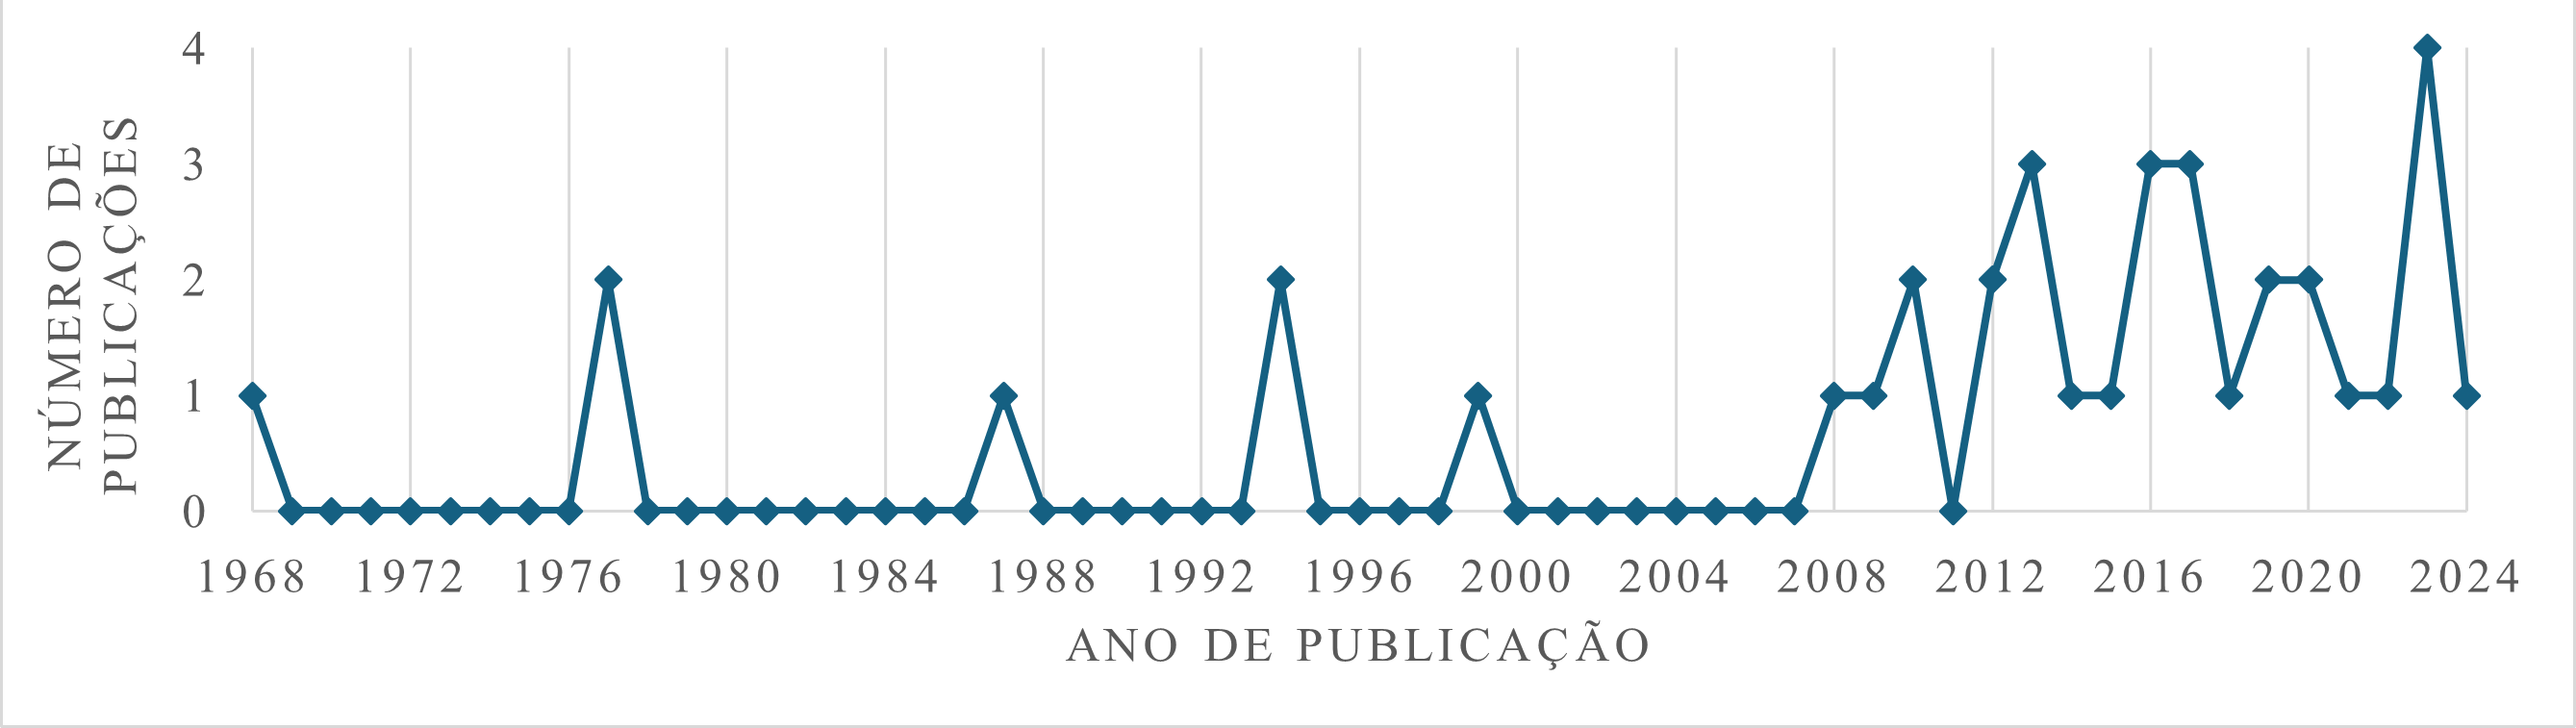
\includegraphics[scale=0.75]{imagens/grafico1.png}
    \fonte{Coleção principal do Web of Science, acesso em maio de 2024.}
    \label{graf:producao_anual}
\end{grafico}

O intervalo encontrado para a produção de artigos sobre FM na WoS foi de 1968 a 2024. Foram encontrados nesse indexador 36 documentos produzidos por 64 autores. A idade média dos textos foi de 13,5 anos, demonstrando que, apesar da frequência com que esses documentos são produzidos ter aumentado a partir de 2008, como é possível observar no Gráfico \ref{graf:producao_anual}, o campo teórico da FM já existe, pelo menos, desde 1968. Os países que mais concentraram publicações foram a Alemanha (11) e os Estados Unidos (10), seguidos pela Holanda (7), Inglaterra (4), México (2), França (1) e Índia (1), demonstrando que o estudo da temática continua concentrado em poucos países. Porém, foi possível observar que há um interesse crescente no estudo da FM.


\section{Fecundidade masculina pelo mundo}\label{tft_tef_mundo}

Cada vez mais há uma percepção de que é relevante compreender os aspectos reprodutivos masculinos, uma vez que a fecundidade masculina possui aspectos específicos, que a distingue da fecundidade feminina. \citeonline{zhang2010male} investigou os diferenciais nas TFTs e das TEFs femininas e masculinas utilizando como fonte principal a publicação \textit{“Demographic Yearbook 2001-Special Topic: Natality Statistics”}\cite{unstatsu25:online2001}. O autor analisou, ao todo, dados de 43 países entre os anos 1990 e 1998, utilizando o intervalo de idade (idade fértil) para as Taxas de Fecundidade Específicas por idade femininas (TEFF) de 15-49 e 15-59 para o cálculo das Taxas de Fecundidade Específicas por idade masculinas (TEFM). A partir de sua pesquisa, \citeonline{zhang2010male} constatou que o coeficiente de variação (CV) para as Taxas de Fecundidade Total Masculinas (TFTM) foi de 0,44, enquanto as Taxas de Fecundidade Total Femininas (TFTF) tiveram o CV de 0,37, indicando uma variação maior nos níveis das TFTMs em relação às TFTFs entre os países analisados. Em seu trabalho, o autor identifica ainda que, em países onde a fecundidade feminina é alta (estabelece TFTF > 2,2), a diferença entre a TFTM e TFTF tende a ser maior, enquanto países com TFTF abaixo desse valor tendem a apresentar taxas comparáveis ou mesmo um nível de TFTF levemente acima da TFTM. Suas conclusões indicam que as TFTMs estão mais espalhadas em relação à média, entre os países analisados, do que as taxas femininas. Ou seja, o número médio de filhos tidos pelas mulheres ao longo de sua vida reprodutiva (nos países analisados) é mais concentrado em torno da média feminina do que o número de filhos tidos por homens em relação a sua média. Adicionalmente, a transição de regimes de alta fecundidade para níveis mais baixos parece influenciar a relação entre fecundidade feminina e  masculina.


 Um segundo trabalho, referência para a área da FM, realiza uma revisão a partir de dados para a idade do pai de 163 países no período por volta de 2011. Nele, \citeonline{schoumaker2019male}, corroborando o que foi encontrado por \citeonline{zhang2010male}, observa que a medida que uma população passa pela transição demográfica, a fecundidade masculina e a feminina se aproximam. O número médio de filhos tidos por mulher variou de 1 a 8 filhos entre os países analisados, enquanto para homens o intervalo encontrado foi bem maior. As TFTMs encontradas pelo autor \footnote{O autor calcula a partir das Taxas de Fecundidade Específicas por idade (TEFs), com 7 grupos etários para mulheres, entre 15 e 49 anos e para homens 13 grupos, entre  15 e 79 anos. } para países da África Subsaariana, foram frequentemente 1,5 a 2 vezes maiores que as TFTFs, combinado com uma população mais jovem e diferenças de idade ao nascimento entre homens e mulheres próximas ou superiores a 10 anos. Enquanto nos países ocidentais, com estruturas etárias mais avançadas, a diferença entre homens e mulheres se mostrou menor, tanto na idade ao nascimento, entre dois e quatro anos, como nas TFTs, com uma razão da TFTM pela TFTF, muitas vezes, inferior a um, ou seja, com a TFTF maior do que a TFTM.

\citeonline{schoumaker2019male} encontra valores mais baixos para a TFTM  nos países europeus, em média entre um e dois filhos, sendo geralmente próximos da TFTF. Os países asiáticos, por outro lado, apresentaram uma variedade maior das TFTMs, com o Japão e a Coreia do Sul apresentando cerca de 1,2 filhos por homem, enquanto outros países do continente apresentam valores bem mais altos, Paquistão (5,1), o Iraque (5,5) e o Afeganistão (6,9). Para os países da América Central e do Sul os valores encontrados foram, no geral, baixos, com o Chile, a Costa Rica e Cuba, variando entre menos de dois filhos, apesar de haver o Haiti como exceção, com TFTM superior a cinco filhos por homem. As TFTMs com valores mais elevados, encontrados pelo autor, se concentraram na África Subsariana, onde, dos 43 países analisados (para essa região), metade possuia uma TFTM superior a 8,5 filhos e um quarto dos países, apresentaram um valor superior a 10 crianças por homem. Seu estudo é eficiente em ilustrar a variabilidade que a fecundidade masculina pode alcançar em diferentes contextos.

Outra contribuição de \citeonline{schoumaker2019male} está em observar que países com alta proporção de mulheres em relações poligínicas\footnote{Estado de um homem que está casado com muitas mulheres. “poliginia”, in Dicionário Priberam da Língua Portuguesa [em linha 2], 2008-2024, https://dicionario.priberam.org/poliginia.} estão relacionados a altos valores para a razão da TFTM pela TFTF. Porém, apesar de ser relevante, a poliginia por si só não se mostrou ser fator explicativo determinante, como o autor chama a atenção, essa diferença costuma estar associada a uma condição necessária à poliginia, a diferença de idade entre os cônjuges numa população com crescimento positivo \apud{pison1986demographic}{schoumaker2019male}.

Nesse sentido, a diferença de idade entre parceiros parece ser um fator importante para os diferenciais na TFT de homens e mulheres. Em trabalho recente, \citeonline{dudel2021male} elencam três possíveis razões para as diferenças encontradas nos valores das taxas de fecundidade masculinas e femininas: 1 - Diferenças de idade entre mães e pais combinado com variação nos tamanhos das coortes; 2 - Diferenças no tamanho das populações feminina e masculina; 3 - Diferenças de gênero no efeito tempo.  

O efeito tempo é uma distorção que pode ocorrer em medidas transversais de fecundidade, como é o caso da TFT. Uma taxa transversal é aquela que mistura eventos de diferentes coortes (ao contrário de taxas que acompanham coortes de maneira longitudinal)\cite{FOZ2021metodos}. Isso faz com que a TFT seja afetada pela experiência de coortes distintas, sendo sensível a mudanças comportamentais temporárias, flutuações de curto prazo que pode ser resultado de um adiamento ou adiantamento momentâneo da fecundidade.

Assim, \citeonline{dudel2021male} propõem que a diferença entre as TFTs masculina e feminina poderia advir de diferenças entre os sexos no  adiamento ou adiantamento da maternidade - paternidade. Segundo os autores, apesar de se observar um padrão geral de pais mais velhos que mães, em diferentes momentos e contextos sociais, alguns fatores, como a revolução de gênero, o aumento do nível educacional entre mulheres, costumam estar associados a um adiamento da maternidade e podem criar condições propícias para a diminuição do intervalo de idade entre parceiros (e.g. pela diminuição da dependência das mulheres em relação à renda do cônjuge).

Embora o adiamento da maternidade seja um tema intensivamente estudado pela demografia no contexto da transição demográfica, relativamente pouca atenção tem sido destinada aos fatores associados ao adiamento da paternidade, com exceção a alguns autores \cite{kyzlinkova2018fatherhood,olah2008sweden,office2009patterns,DenmarkNordfalk} que, no geral, têm mostrado o efeito tempo para os homens, da postergação da idade média ao nascimento, tende a acompanhar o das mulheres, porém muitas vezes se mostrando menos atenuado\footnote{\citeonline{DenmarkNordfalk} encontra um efeito tempo negativo para homens e mulheres dinamarqueses entre 1980-2010, com o efeito para as mulheres, mais evidente do que para os homens}. \citeonline{dudel2021male} chegam a conclusão de que as diferenças no adiamento da idade média ao nascimento entre os sexos e a diferença de idade entre parceiros são fatores relevantes para os diferenciais nas TFTs entre os sexos, apontando para tópicos de pesquisa vitais para o campo da FM. 

No que diz respeito às diferenças no tamanho das populações feminina e masculina, ocorre impacto sobre o denominador no cálculo das TEFs, a população exposta. Por exemplo, se a proporção de homens emigrantes de determinado país é maior que a de mulheres emigrantes, a população masculina diminui, podendo temporariamente aumentar a taxa de fecundidade masculina em relação à feminina. 



\begin{comment}

A combinação de diferentes idades entre mães e pais com a variação nos tamanhos das coortes produz discrepâncias na fecundidade de homens e mulheres porque, se homens e mulheres forem de coortes diferentes e houver variação no tamanho das coortes, o denominador das taxas masculinas e femininas podem diferir. \citeonline{schoumaker2017measuring}, por exemplo, demonstrou em países com altas taxas de crescimento populacional a TFTM cresce mais do que a TFTF, já que os pais costumam vir de coortes menores e de idade mais avançadas do que suas parceiras. 




   -----------------------
     A nossa segunda conclusão principal é que as diferenças de idade entre pais e mães permaneceram constantes ou diminuíram na maioria dos países do nosso estudo, exceto nos países da Europa Oriental e na Alemanha Oriental. Embora esta tendência geral esteja em linha com as expectativas baseadas nas teorias de género, as diferenças que existem actualmente entre os países parecem ser afectadas por mais factores do que apenas diferenças nos níveis de igualdade de género.
    -------------- 


Razão de sexo\footnote{Expressa pelo número de homens para cada grupo de
100 mulheres, na população residente em determinado espaço geográfico, no ano
considerado \cite{rede2002indicadores}.}


encontraram indícios de que as mudanças na razão entre a TFTM e a TFTF são governadas pelas diferenças de idade entre parceiros e em mudanças no comportamento reprodutivo, como adiamento da paternidade e maternidade. Analisaram dados de 17 países de renda alta, no intervalo entre 1968 a 2016 ou 1980 a 2016, para a maioria dos países, e chegaram a algumas conclusões interessantes. Segundo os autores,\textbf{o adiamento da maternidade e da paternidade são fatores...}


From a demographic perspective, such disparities can be driven by three main factors: first, differences in the population sizes of males and females, i.e., in the sex ratio, which can affect both TFR and CFR differences; second, age differences between mothers and fathers in interplay with variation in cohort sizes (affecting the TFR and the CFR); and, third, gender differences in tempo effects, which can impact gender differences in the TFR, but not in the CFR.



---
\textbf{quando os pais são atribuídos à mesma coorte que as mães, e que grandes diferenças de gênero nos níveis de fecundidade são muitas vezes motivadas por diferenças no momento da fecundidade. }


EM WONG 2020- SOBRE SCHOUMAKER 2019:

    The author shows that the TFR of men is almost always higher than that o

women, which he explains by two factors. The first is that men have a higher mortality rate than women, which would lead to fewer men exposed to the risk of parenthood. The second is that men tend to bond and have children with women younger than themselves. If these cohorts of men and women were born in a context of positive population growth, then the cohort of men tends to be smaller than that of women, also decreasing the population at risk of paternity.
\end{comment}

%Taxas Específicas de Fecundidade por idade

Quando falamos do padrão masculino da fecundidade nas faixas etárias, \apudonline{paget1994relational}{zhang2010male}, ao observar países com distintos níveis de TFT nas décadas de 1960-80, identificaram que os homens teriam, em geral, o início de sua vida reprodutiva postergado e uma parada bem posterior em relação às mulheres. Os homens teriam um pico mais tardio e inferior, com as TEFMs permanecendo mais elevadas do que as TEFFs em faixa-etárias mais avançadas. 

\citeonline{zhang2010male} subdivide a análise, com dados para os anos de 1990 a 1998, das TEFs entre países com TFT feminina alta e baixa (TFTM < 2,2 e TFTF < 2,2). O autor encontra que as TEFFs superam as TEFMs nas faixas etárias mais jovens (15–19, 20–24 e 25–29), com o valor médio da TEFFs da faixa etária de 15-19 anos sendo até cinco vezes maior que as TEFMs para esse grupo etário, tanto em países com alta, como com baixa TFT. A faixa de 30 a 34 anos se mostrou um ponto de inflexão na relação da fecundidade masculina com a feminina, sendo observado que nessa faixa as TEFMs começam a superar os níveis das TEFFs, com a razão da TEFM pela TFTF próxima de um. 

{\citeonline{zhang2010male} avança ao descobrir que um fator de mudança na correlação das TEFs feminina e masculina é quando as TFTs se aproximam do nível de reposição demográfica (2,2), quando a TFTM costuma alcançar um patamar inferior a TFTF. As hipóteses que o autor levanta sobre essa questão estão associadas ao denominador no cálculo das taxas de fecundidade, ou seja, mudanças no número de homens na faixa etária. O fato de países com TFT abaixo do nível de reposição serem, geralmente, países de economia desenvolvida pode estar associado a níveis altos de imigração, com o inverso verdadeiro, altas TFTs associadas a menor desenvolvimento e alta emigração. Compreendendo a migração como um movimento feito majoritariamente por homens jovens, isso contribuiria para que o denominador ficasse maior (e uma menor TFTM) em países desenvolvidos e menor em países menos desenvolvidos (TFTM maior). A segunda hipótese, também atrelada aos níveis de desenvolvimento, foca nos diferenciais de mortalidade por sexo. As mulheres costumam desfrutar de uma expectativa mais longa e menores níveis de mortalidade do que homens. O autor conjectura que, em países desenvolvidos, a expectativa de vida masculina pode ser maior e os níveis de mortalidade masculinos menores. Porém, apesar das hipóteses, deixou em aberto o motivo pelo qual a correlação entre TFTM e TFTF se modifica no ponto em que os países alcançam a TFTs no nível de reposição.

\begin{comment}
- diferenças de idade na parturição ---
\cite{dudel2021male}:
----Embora observemos padrões bastante diversos nas diferenças de idade entre países e grupos de países, o mecanismo demográfico subjacente é, em todos os casos, diferenças de gênero no adiamento. Especificamente, em todos os países que estudamos, a idade média ao dar à luz tem aumentado continuamente desde 1990, tanto para homens como para mulheres (ver materiais suplementares para obter detalhes); ou seja, tanto homens como mulheres têm adiado o parto. Em combinação com uma idade média de parto mais elevada para os homens, esta conclusão sugere que as mudanças na diferença de idade parental no momento do parto se devem a diferenças na velocidade com que o adiamento avança: se progredir mais rapidamente entre os homens do que entre as mulheres, a diferença de idade aumenta; mas se, por outro lado, avança mais rapidamente entre as mulheres do que entre os homens, a diferença de idade diminui----

tefs - United Nations Demographic Yearbook 2021




POP ESTÁVEL  (schoumaker)
    Em contraste, os países ocidentais combinam baixas diferenças de idade entre parceiros e estruturas etárias mais avançadas. Ambos os factores estão em jogo nas diferenças entre homens e TFRs femininas, como será demonstrado no caso de populações estáveis. 



IMIGRAÇÃO: (schoumaker)

    O efeito da migração internacional é visível em alguns países onde a razão é muito inferior ao esperado devido à diferença de idade (por exemplo, no Bahrein e no Qatar, com grande imigração masculina), ou superior ao esperado em países com grande emigração masculina, como no Nepal com o DHS. Em contraste, as estimativas que corrigem a migração internacional (seja no Nepal ou no Qatar) estão mais em linha com outras estimativas.

    (ZHANG)
When the cumulative pattern of fertility is considered, male total fertility rates (TFRs) are found to be different from those of females. It is shown that male TFRs were first higher than female TFRs in most Western industrialized countries before the 1960s. Such male and female fertility differentials are likely to be resulted from the relative shortage of men caused by two world wars. Since the 1960s, males in most industrialized countries have recovered from war time losses. Coupled with an increasing emigration that has been replaced by immigration which is largely dominated by men, male TFRs turned to be higher than female TFRs afterwards (Coleman, 2000). In addition to male and female fertility differentials in rates, demographers have also indicated that the progeny size distribution and childlessness patterns of men and women differentiate male fertility from female fertility.

\end{comment}


\begin{comment}
    A nossa segunda conclusão principal é que as diferenças de idade entre pais e mães permaneceram constantes ou diminuíram na maioria dos países do nosso estudo, exceto nos países da Europa Oriental e na Alemanha Oriental. Embora esta tendência geral esteja em linha com as expectativas baseadas nas teorias de gênero, as diferenças que existem atualmente entre os países parecem ser afetadas por mais factores do que apenas diferenças nos níveis de igualdade de gênero. Embora as nossas descobertas indiquem que a fecundidade masculina tem sido geralmente inferior à fecundidade feminina nos últimos anos, esta tendência não parece manter-se a nível mundial. 

    Schoumaker (2017, 2019) mostrou que em contextos em que a poliginia é praticada e as populações estão a crescer rapidamente, os níveis de fecundidade masculina podem por vezes ser duas vezes superiores aos níveis de fecundidade feminina. Seus resultados sugerem que esse padrão é impulsionado, em grande parte, pelas diferenças de idade entre os casais. 
    
    Esta conclusão está em linha com os resultados da nossa análise contrafactual, que indicam que os casos extremos tendem a desaparecer quando os pais são atribuídos à mesma coorte que as mães, e que grandes diferenças de gênero nos níveis de fecundidade são muitas vezes motivadas por diferenças no momento da fecundidade. . No outro extremo, o razão TFT mais baixo relatado na literatura é para Inglaterra e País de Gales em 1973, em torno de 0,89 (Schoen 1985). O valor que encontramos para a Alemanha Oriental, 0,84, está abaixo deste nível e pode indicar que os homens da Alemanha Oriental têm experimentado o que Schoen (1985) chamou de “aperto de natalidade”: ou seja, na Alemanha Oriental, o número desigual de homens e mulheres na faixa etária reprodutiva está tendo impacto na fecundidade dos homens. Geralmente, a variação nas razões TFR que observamos entre países e ao longo do tempo não é negligenciável. Os grupos de países com semelhanças culturais e/ou políticas parecem ter padrões de tendências mais semelhantes. Esta descoberta requer uma investigação mais aprofundada.




---- 
dudle 2016: 

as diferenças de idade dos pais aumentaram para as mães mais jovens e diminuíram para as mães mais velhas; e a heterogeneidade entre as faixas etárias aumentou. As inclinações para os homens apresentam menos variação do que as inclinações para as mulheres. 

na perspectiva dos pais, as diferenças de idade entre os pais têm geralmente diminuído, mas também tem havido um padrão bastante estável de pais mais velhos que tendem a ter filhos com mães muito mais jovens.

“observations that men generally prefer younger partners as they become older, while women’s age preferences for their partners are more heterogeneous (Skopek, Schmitz, and Blossfeld 2011).” ([Dudel et al., 2020, p. 13](zotero://select/library/items/XGG8CKCJ)) ([pdf](zotero://open-pdf/library/items/54XEELWP?page=14\&annotation=LPQ2UYNK))

a mudança nas diferenças de idade dos pais ao longo do tempo foi influenciada pelo género. Para as mulheres, esta mudança levou a uma maior heterogeneidade entre idades, de tal forma que as diferenças de idade dos pais entre mães mais jovens e mais velhas diferem mais hoje do que no passado. Entre os pais, por outro lado, as diferenças de idade parentais diminuíram, independentemente da idade em que tiveram um (outro) filho. Estas observações estão em linha com as conclusões existentes de que as alterações na fecundidade por estatuto social ou por idade que ocorreram nas últimas décadas foram muito maiores para as mulheres do que para os homens (ver Jalovaara et al. 2018). Uma possível explicação para isto é que o estatuto socioeconômico das mulheres tem vindo a mudar mais rapidamente. No entanto, embora seja claro que os padrões de disparidades de idade dos pais são de gênero, os resultados das nossas análises de regressão indicam que a diminuição das diferenças de idade dos pais que são atribuíveis ao atraso na parentalidade apresenta regularidades notáveis entre países ao longo do tempo.

indicam que, para as mulheres, o parto mais tardio está associado a uma menor diferença de idade parental; e, portanto, com uma relação de poder mais equilibrada. Nas últimas décadas, detectamos que as mães mais jovens têm filhos com parceiros cada vez mais velhos, o que sugere que é cada vez mais provável que estejam numa união com relações de poder desiguais. Para os pais, o parto mais tardio está associado a uma maior diferença de idade parental, o que implica que estes tenham maior poder na relação. No entanto, este efeito tem diminuído ao longo do tempo à medida que o adiamento da fecundidade aumentou entre homens e mulheres.” ([Dudel et al., 2020, p. 13]


\end{comment}

\begin{comment}

FATORES SOCIOLÓGICOS, ESTUDOS DE GÊNERO E PREFERENCIAS REPRODUTIVAS ENTRE HOMENS E MULHERES: 
\begin{itemize}
    \item Challenging Demography: Contributions from
Feminist Theory (Nancy E. Riley)
    \item Masculinity: An Overlooked Cultural Influence on Fertility
Rachael S. Pierotti, University of Michigan
\end{itemize}


SOCIOLOGICO (zhang) 
    Beyond investigating fertility determinants, examining other dimensions of fertility needs involving males as well. For example, understanding the timing of parenthood demands exploring closely the meaning of fatherhood and motherhood in various cultural institutions and how the meaning changes over the life course for men as compared to for women. Looking into the link between the construction and deconstruction of a childbearing and childrearing union (such as cohabitation and marriage) also requires knowing more about men’s commitment in these unions. The women’s health movement has also stressed the need for men to be aware of their responsibilities in family planning and reproductive health. In sum, it is imperative to bringing men into fertility and fertility-related research. Male fertility should be considered as an important component of fertility studies.


https://citeseerx.ist.psu.edu/document?repid=rep1&type=pdf&doi=db7234060968eb15b6239c3661d5dcac5159c3a5 
    Este artigo demonstra que a educação influencia o comportamento reprodutivo dos homens de múltiplas maneiras. Centrando-nos particularmente na falta de filhos e na fecundidade multiparceira, os elementos-chave nas nossas análises são factores relacionados com a capacidade de um homem para uma parentalidade económica e prática, reflectida, por exemplo, na sua capacidade parental. através das perspectivas de rendimento, da segurança no emprego, da flexibilidade laboral e da composição de género do emprego.

\citeonline{goldscheider1996fertility}





- estudos atuais(relevancia atual):  \cite{keilman2014measures}, \cite{gerber2014two}


\section{referencias do Zhang -- antigas:}

\begin{itemize}
  
    \item Os efeitos da idade na fecundidade masculina e feminina também são muito diferentes. As mulheres atingem seu pico de fecundidade entre 25 e 35 anos, após o qual a fecundidade começa a declinar até a menopausa. Já os homens continuam a ter capacidade reprodutiva até a morte, embora de forma gradual (Wood, 1994). 
    \item Quando o padrão cumulativo de fecundidade é considerado, as taxas de fecundidade total masculina (TFR) são encontradas como diferentes das femininas. Observa-se que as TFR masculinas eram maiores que as femininas na maioria dos países industrializados ocidentais antes dos anos 1960.
        \begin{itemize}
            {\item Essas diferenças de fecundidade entre homens e mulheres provavelmente resultaram da relativa escassez de homens causada pelas duas guerras mundiais. Desde os anos 1960, os homens na maioria dos países industrializados recuperaram-se das perdas da guerra. Aliado ao aumento da emigração substituída pela imigração predominantemente masculina, as TFR masculinas passaram a ser maiores que as femininas (Coleman, 2000)}
       \end{itemize}
    \item Além das diferenças nas taxas de fecundidade entre homens e mulheres, demógrafos também indicaram que a distribuição do tamanho da prole e os padrões de ausência de filhos diferenciam a fecundidade masculina da feminina. Algumas pesquisas mostram que, em geral, os homens têm menos filhos que as mulheres. 
    Consequentemente, há percentagens mais altas de homens sem filhos em comparação com as mulheres (Coleman, 2000). Todos esses fatos sugerem que a fecundidade humana não pode ser totalmente representada pela fecundidade feminina. Usar as taxas de fecundidade feminina para representar as masculinas pode ser problemático, especialmente em sociedades onde as taxas de divórcio, novo casamento e migração são bastante altas. Pesquisadores sugerem que mesmo aplicar as taxas de fecundidade feminina marital para representar a fecundidade humana como uma solução alternativa é inadequado, pois as taxas de nascimentos não maritais em algumas sociedades são comparativamente altas e os homens têm mais probabilidade de se casar novamente após o divórcio do que as mulheres, o que torna a fecundidade masculina e feminina não comparável (Greene \& Biddlecom, 2000; Juby \& Bourdais, 1998; Magnani, Bertrand, Makani, \& McDonald, 1995).

    \item Além de investigar os determinantes da fecundidade, examinar outras dimensões da fecundidade também exige envolver os homens. Por exemplo, entender o momento da paternidade exige explorar de perto o significado da paternidade e maternidade em várias instituições culturais e como o significado muda ao longo da vida para homens em comparação com mulheres. Analisar a ligação entre a construção e desconstrução de uma união de criação de filhos (como coabitação e casamento) também requer saber mais sobre o compromisso dos homens nessas uniões. O movimento pela saúde da mulher também destacou a necessidade de os homens estarem cientes de suas responsabilidades no planejamento familiar e na saúde reprodutiva. Em suma, é imperativo incluir os homens nas pesquisas de fecundidade e relacionadas à fecundidade. A fecundidade masculina deve ser considerada um componente importante dos estudos de fecundidade.
\end{itemize}






-----------
\end{comment}
\section{Principais bases e métodos}\label{bases_e_metodos-ref}


A TFT e as TEFs são geralmente calculadas para mulheres, porém, como defendemos aqui, ambas podem e devem ser calculadas também para homens. As TEFs por idade (${}_n{f}_x$, onde $x$ é o limite inferior da faixa de idade e $n$ o tamanho do intervalo, geralmente intervalos quinquenais de idade) relacionam-se ao número de nascimentos ocorridos entre homens de uma determinada idade ou grupo etário com o tempo total de exposição dos mesmos ao risco de terem filhos naquele mesmo período \cite{FOZ2021metodos}. Definida por:

\begin{equation}\label{tefmEqu}
{}_n{f}_x = 1000 \cdot \frac{\text{\footnotesize \textit{Número de nascimentos ocorridos aos homens com idades entre} } x \text{ \footnotesize e } x + n \text{ \footnotesize \textit{no período}}}{\text{\footnotesize \textit{População média de homens com idades entre} } x \text{ \footnotesize e } x + n \text{ \footnotesize \textit{no período}}} \\
\end{equation}

Já a TFTM quantifica o número médio de filhos nascidos vivos que um homem teria ao longo dos seus anos reprodutivos, se fosse exposto às TEFs masculinas de um determinado ano. Como vimos anteriormente\footnote{Seção \ref{tft_tef_mundo}}, a TFT pode ser afetada quando ocorre um adiamento ou adiantamento da paternidade-maternidade. Porém, é um dos indicadores mais relevantes para caracterizar o nível da fecundidade da população de determinado território ou grupo social. É obtido somando as TEFs (${}_n{f}_x$) e multiplicando pela amplitude do grupo etário $n$, onde $\alpha$ e $\beta$ indicam o início e o fim do intervalo reprodutivo masculino:

\begin{equation} \label{tftEqu}
TFT = n \sum_{x=\alpha}^{\beta} {}_n{f}_x
\end{equation}


Não há consenso sobre o intervalo utilizado para o período reprodutivo masculino, sendo utilizados diferentes intervalos entre os autores (15-59, 15-79, 17–59, 15-50, 15-59, 20-59\footnote{\citeonline{zhang2010male,schoumaker2019male,dudel2016estimating, kyzlinkova2018fatherhood, unstatsu2022Nota} e \citeonline{office2009patterns}, respectivamente. Alguns autores adotam intervalos diferentes conforme limitações da base de dados.}). A maioria dos autores agrupa os nascimentos observados fora do limite superior e inferior nas coortes limites. Por exemplo, considerando nascimentos com idade masculina observada menor de 14 anos, parte do grupo etário 15-19 anos. Nascimentos abaixo de 15 anos e acima de 60 costumam ser apontados como eventos rarefeitos.  
  

Conforme vimos a partir de \citeonline{zhang2010male}, os estudos de fecundidade masculina têm como uma de suas principais barreiras, a qualidade dos registros para idade do pai ao nascimento, informação necessária para se obter o numerador do cálculo das TEFMs (equação \ref{tefmEqu}). Os dados de fecundidade masculina estão disponíveis em muitos países ocidentais através do registo civil e sistemas de estatísticas vitais (CRVS). O \textit{“United Nations Demographic Yearbook”} compila o número de nascidos vivos por idade do pai e calcula as TEFMs através de registros civis e é uma das principais bases que tem sido utilizadas para os estudos de fecundidade masculina pelo mundo. A publicação é baseada em dados coletados das autoridades nacionais de estatística de diversos países, desde 1948. Ela é considerada uma das bases mais completadas que contém informação sobre fecundidade masculina, apresentado dados nas edições de 1949–1950, 1954, 1959, 1965, 1969, 1975, 1981, 1986, 1999 e 2007-2022 \cite{unstatsu25:online}. Porém, a base possui limitação quanto a sua abrangência. Sendo composta majoritariamente por nações onde os CRVS são mais avançados \cite{zhang2010male} e atingem maior completude, ou seja, com baixa proporção de dados faltantes. Essa foi a principal fonte de informação utilizada nas análises de \citeonline{zhang2010male} e \citeonline{paget1994relational}. 

Visando ampliar a análise da fecundidade masculina para países não abarcados pelo \textit{“United Nations Demographic Yearbook”}, \citeonline{schoumaker2017measuring} elabora e compara três métodos para estimar as TEFMs utilizando as bases do \textit{“Demographic and Health Surveys (DHS)”}\footnote{Pesquisa de saúde realizada a mais de 30 anos em cerca de 90 países. Dentre as informações coletadas (sobre mortalidade infantil, fecundidade, planejamento familiar, saúde materna, imunização infantil, níveis de desnutrição, prevalência do HIV e malária) estão aspectos relacionados a fecundidade e reprodução masculina. Fonte: https://www.usaid.gov/global-health/demographic-and-health-surveys-program.}. As pesquisas do programa DHS se estruturam por três questionários, aplicados aos moradores, à mulher selecionada (entre 15-49 anos) e ao homem selecionado (geralmente entre 15-59 anos). O autor utiliza os dados disponíveis para encontrar o número de nascimentos ocorridos aos homens nas faixas idades. Os três métodos utilizados foram: método dos filhos próprios \textit{(own-children method)}, o método da data do último nascimento \textit{(the date-of-last-birth method)} e o método cruzado \textit{(the crisscross method)}.



O método dos filhos próprios (MPF), utilizado habitualmente para calcular a fecundidade feminina, foi adaptado pelo autor para o caso dos homens mediante basicamente cinco passos: parear a criança sobrevivente com o respectivo pai, classificar os filhos por idade e por idade do pai em dado ano, redistribuir as crianças não correspondidas por idade do pai, reverter a sobrevivência das crianças para estimar o número de nascimentos por ano e idade do pai nos anos anteriores ao levantamento, e  reverter a sobrevivência da população masculina nos anos anteriores à pesquisa para estimar o denominador das TEFMs \cite{schoumaker2017measuring}. 
Formalmente, a TEFM no período entre $x$ e $x+1$ anos antes do momento da pesquisa, para homens que naquele momento tinham entre $y-x-1$ e $y-x$ anos deve ter sido: 

\begin{equation}
    TEFM_{y-x}(t-x-\text{\footnotesize1/2})=P_{x,y}\frac{\ell_{0}}{\ell_{x+\frac{1}{2}}} / P_{y}\frac{\ell_{y-x}}{\ell_{y+\frac{1}{2}}}
\end{equation}

No numerador temos ($P_{x,y}$) filhos atualmente vivos (sobreviventes dos que nasceram num momento passado), crianças de $x$ anos completos de idade cujos pais têm $y$ anos, multiplicado pela razão de sobrevivência da criança no intervalo ($P_{x,y} \ell_{0} / \ell_{x+\frac{1}{2}}$). O denominador é composto pelos pais atuais, sobreviventes dos que haviam na época, através de $P_{y}$ $\ell_{y-x} / \ell_{y+\frac{1}{2}}$ \cite{FOZ2021metodos}.  

Para o primeiro passo, parear as crianças sobreviventes aos seus respectivos pais (para obter idade dos pais ao nascimento), \citeonline{schoumaker2017measuring} utiliza informações inclusas nos próprios dados da DHS, disponíveis para quando ambos residem na mesma casa. Para o caso no qual o pai vive em casa diferente, o autor estimou as idades dos pais sobreviventes utilizando por registro doador (Hot-Deck) \apud{allison2001missing}{schoumaker2017measuring}, retirando crianças sobreviventes que relataram que seus pais não eram mais vivos. 
A idade do pai para os filhos cujo pai está vivo foi então imputada para cada filho não pareado, um filho com as mesmas características (idade e idade da mãe) foi selecionado aleatoriamente entre os filhos pareados\footnote{O autor realizou a imputação aleatória 10 vezes e calculou 10 séries das TEFMs, considerando, ao final, a média das 10 séries de TEFMs}.
A idade do pai do filho selecionado foi então atribuída ao pai do filho sem correspondência.
O autor afirma que se seguisse a abordagem padrão para o MFP (normalmente aplicado para o cálculo das TEFF), iria supor a mesma distribuição de idade dos pais de filhos compatíveis e de filhos não correspondidos de idade $x$, usar a idade da mãe no processo de imputação levou a uma idade ao nascimento mais baixa (um ano em média) para pais de filhos não correspondidos em comparação com pais de filhos pareados. Em seu processo de estimação, o autor encontrou que outras informações poderiam ser consideradas no processo de imputação, como o tipo de local de residência, porém demonstraram ter um impacto limitado nos resultados. 

Em seguida, para encontrar um pai (de idade imputada) para filhos não pareados, um homem com a mesma idade que a idade imputada do pai  foi selecionado aleatoriamente entre os homens no conjunto de dados do agregado familiar, independentemente do homem já ser pai ou não. Os últimos passos foram, estimar o número de nascimentos em $x$ anos antes da pesquisa (através do inverso da probabilidade de sobrevivência dos filhos com idade completa $x$) para, por fim, calcular as TEFMs, os nascimentos durante os cinco anos anteriores à pesquisa são somados por faixa etária dos pais ao nascimento, e a exposição é obtida somando o tempo que cada homem passou em cada faixa etária nos últimos cinco anos.

O segundo método proposto por \citeonline{schoumaker2017measuring} foi o da data do último nascimento. Nele, é pressuposto que as TEFMs são constantes para o grupo etário $j$ em dado período. As taxas de fecundidade no grupo etário $j$ ($\lambda_{j}$) são calculadas como a razão entre o número de nascimentos visíveis (últimos nascimentos) no grupo de idade $j$ e a exposição dos homens nessa faixa etária naquele período, medido como a soma da duração (para cada homem) passada na faixa etária entre a data do inquérito e a data do último nascimento, ou a data do início do período, se nenhum nascimento ocorreu durante o período (faixa do grupo etário, por exemplo, cinco anos). No método não é possível captar caso tenha ocorrido mais de um nascimento para o pai durante o período, o que gera subestimação da fecundidade. Porém, uma vantagem dessa escolha, segundo o autor, é de que seria possível  analisar as TEFMs entre diferentes grupos, com seus marcadores sociais ou características como tipo de relação monogâmica-poligínica, isso porque o número de nascimentos visíveis por grupo etário 
 é uma informação obtida diretamente do questionário dos homens selecionados.  


\begin{equation}
   TEFM (\lambda_{j}) = \frac{\text{\footnotesize \textit{número de nascimentos visíveis por grupo etário} }j}{\text{\footnotesize \textit{exposição visível no grupo etário}}j}
\end{equation}


Na terceira e última abordagem exposta por \citeonline{schoumaker2017measuring}, o método cruzado, é feito uma comparação entre os dados das crianças nascidas vivas em duas edições da DHS. TEFMs ($\lambda$) entre duas idades $x$ e $x+n$ sobre um período ($t$) são estimadas pela equação “crisscross”\footnote{Para maiores detalhes ver o trabalho \textit{“The crisscross method to evaluate data quality in fertility surveys”}\cite{schoumaker2014crisscross}, onde o autor detalha melhor seu método.}. Utiliza-se o número médio de crianças já nascidas por idade exata, estimado suavizando o número de crianças já nascidas por idade completa. As vantagens desse método seria que, por se basear no número de crianças já nascidas, não seria afetado por imprecisões nas datas de nascimento ou idades das crianças. No entanto, seria impactado por omissões diferenciais de nascimentos nos inquéritos e diferenças na composição da amostra entre edições da DHS (e.g. se homens com fecundidade elevada forem sub-representados).

A principal contribuição do trabalho de \citeonline{schoumaker2017measuring} é possibilitar a estimação da fecundidade masculina em países onde os registros administrativos não são totalmente consolidados. O Brasil tem bases da DHS para os anos de 1986, 1991 e 1996, disponíveis no site do programa DHS \footnote{Fonte: \href{https://dhsprogram.com/Countries/Country-Main.cfm?ctry_id=49\&c=Brazil}{Programa DHS - Brasil.}}, porém, em 1991, foi realizada uma pesquisa de Demografia e Saúde da Mulher e da Criança com abrangência somente para o Nordeste\footnote{\href{https://dhsprogram.com/publications/publication-FR5-DHS-Final-Reports.cfm}{Relatório Final - Pesquisa sobre Saúde Familiar no Nordeste Brasil 1991}}. Em 2006, foi realizada a Pesquisa Nacional de Demografia e Saúde da Criança e da Mulher (PNDS) nos moldes da 5ª fase do projeto DHS e está previsto para 2025 o resultado da PNDS de 2023, baseado na 8ª rodada do programa. A PNDS 2023 será a primeira a fornecer histórico de filhos biológicos nascidos vivos, para homens entrevistados de 15 a 59 anos, informação que poderá ser utilizada para cálculo da fecundidade masculina. As edições de 1991 (com abrangência para o Nordeste) e de 1996 tiveram questionários aplicados ao 'marido' e ao homem selecionado.  

\citeonline{wong2020LatinA} estimam as TEFMs e a TFTM utilizando métodos indiretos a partir de microdados disponíveis na plataforma do \textit{“Integrated Public Use Microdata Series (IPUMS), International”}, dos censos do Brasil, Argentina, Chile, Colômbia, Equador, México, Paraguai, Uruguai e Venezuela desde 1970. O método utiliza informações sobre a composição familiar e assume que o cônjuge ou companheiro da mulher que teve um filho nascido vivo nos 12 meses anteriores ao censo é o pai da criança. A partir do quesito que pergunta às mulheres sobre nascidos vivos nos últimos 12 meses ou pela idade do filho mais novo, calcula-se a fecundidade de período para os homens. Para estimar as idades dos pais ausentes (mulher solteira), os autores utilizaram a imputação condicional à idade da mãe, na qual a idade do pai-cônjuge ausente é a média de idade dos pai-cônjuges observados $b$ das mulheres em idade $a$, em cada país e ano \cite{wong2020LatinA}. 

\begin{equation}
    \hat{b} = E[b|A=a]
\end{equation}

As TEFMs foram obtidas pela divisão do número de nascimentos, pelo número de homens, no grupo etário. Os autores, buscaram corrigir possíveis fontes de erro (erro no registro do período de referência, subestimação do número de crianças na casa) a partir de um fator de correção, comparando a TFT feminina calculada pelo método indireto do artigo com a estimada pelo \textit{UN World Prospects\footnote{\href{https://population.un.org/wpp2019/}{World Population Prospects 2019.}}} (mantendo o padrão etário da população de cada país no momento do censo).     

Houve alguns autores que tentaram contornar o problema da qualidade dos registros administrativos e estimar a fecundidade masculina em países onde havia uma proporção considerável de dados faltantes. No Brasil, \apudonline{Wong1986}{wong2022fecundidade} usaram dados administrativos para calcular a fecundidade
masculina em São Paulo(SP) em 1983. Reportaram que, à época, cerca de 10\% dos registros de nascimento estavam com a idade do pai como “ignorada”. Infelizmente não consegui acesso ao artigo original das autoras para verificar se foram utilizadas técnicas de imputação. 

\citeonline{falcao_fecundidade_2013} utilizou microdados do Sistema de Informação sobre Nascidos Vivos (SINASC) e informações do Sistema Estadual de Análise de Dados - SEADE (para o denominador, distribuição da população por sexo e idade) para estimar a TFTM e as TEFMs para alguns municípios de SP. O critério de seleção dos municípios no artigo foi aqueles que possuíam um registro superior a 1.500 nascimentos no ano, e aqueles nos quais os registros com idade do pai não declarada fossem inferior a 8,0\%. Apenas 14 municípios paulistas do ano selecionado (2013) cumpriram os dois critérios. O autor limita, em sua análise, o período reprodutivo masculino de 15 aos 59 anos, após observar que os registros com pais acima de 60 anos não eram suficientemente robustos para alterar a TFTM. Em sua análise, \citeonline{falcao_fecundidade_2013} utiliza apenas os registros que possuem idade do pai observada, deletando os registros com idade do pai ausente.    

\citeonline{dudel2019estimating} utilizam registros administrativos da
Suécia (1968-2014), EUA (1969-2015), Espanha (1975-2014) e Estônia (1989-2013), onde a idade do pai é faltante em cerca de 1\%, para a maioria dos anos na Suécia, mas chegou a 17\% no início da década de 1990 nos EUA. Os autores problematizam a abordagem utilizada por alguns autores para lidar com o problema dos dados faltantes para a idade do pai, adotada também pelo “United Nations Demographic Yearbook”\cite{unstatsu2022Nota}. Normalmente os nascimentos de pais de idade desconhecida são distribuídos proporcionalmente pelas faixas etárias, de acordo com a distribuição dos nascimentos por idade do pai antes do cálculo das taxas. Dessa forma, é pressuposto que a idade do pai é ausente por motivos totalmente aleatórios e que a distribuição das idades não registradas é a mesma das observadas. \citeonline{dudel2019estimating} discordam dessa abordagem e comprovam, através da simulação de 71.550 cenários, que a imputação das idades paternas faltantes condicionada pela idade da mãe observada tem um melhor desempenho na grande maioria das simulações.  

Em seu trabalho, \citeonline{dudel2019estimating} distribuem as idades do pai não observadas de duas maneiras, condicional e não condicional à idade da mãe (assumida como sempre observada), e testam, ao final, qual das duas abordagens apresenta melhor desempenho, estimando as TEFMs para os países em determinado ano. Onde $B(x,t)$ denota os nascimentos de homens em idade $x$ no tempo $t$, $N(x,t)$ referencia a população exposta de homens em idade $x$. A TEFM calculada, como anteriormente, pelos nascimentos sobre a população exposta é dado por: $f(x,t)=B(x,t)/N(x,t)$, retirando-se o índice $t$ para simplificar as fórmulas. $B(\ast)$ representa o número de nascimentos com idade do pai desconhecida e $B^*(x)$ os nascimentos com idade do pai observada. 


Na abordagem incondicional, $B(\ast)$ (idades não observadas) são distribuídas conforme as idades observadas $B^*(x)$ e $P^*(x)$ é a proporção de pais em idade $x$ calculada ignorando valores ausentes. O cálculo da TEFM é expresso da seguinte forma: 

\begin{equation}
    f(x)=\frac{B^*(x)+B(\ast)P^*(x)}{N(x)}
\end{equation}

Para a abordagem condicional, considera-se $B^*(x,y)$ o número de nascimentos de pais em idade $x$ e mães em idade $y$. $P^*(x|y)$ é a distribuição da idade paterna condicional à idade da mãe, a partir dos valores observados para idade do pai, calculados: $B^*(x,y)/ \sum_{i=\alpha}^{\beta}B^*(i,y)$, onde $\alpha$ e $\beta$ representam a primeira e a última idade reprodutiva dos homens; $B(\ast,y)$ representa o número de nascimentos para os quais a idade materna é conhecida e igual a $y$ e a idade paterna é desconhecida. Assim, pela abordagem condicional, a TEFM é calculada (onde $\gamma$ e $\delta$ denotam as idades mais nova e mais velha das mulheres): 

\begin{equation}
    f(x)=\frac{B^*(x)+\sum_{j= \gamma}^{\delta}  B(\ast, j)P^*(x|j)}{N(x)}
\end{equation}





\begin{comment}

(fazer uma tabela mostrando os métodos já propostos e as bases utilizadas, seus pós e contra --\textit{shoumaker})


problema do método de estimar pelos filhos que coabitam residencia com os pais: 
mudanças no padrão de casamento, multiparentalidade--- >

https://journals.library.ualberta.ca/csp/index.php/csp/article/view/15837/12642
.....

FECHAR FALANDO SOBRE O PORQUE ESCOLHER A METODOLOGIA QUE ESCOLHI PARA TRATAR O DADO... 

\end{comment}





\section{Fecundidade masculina no contexto brasileiro}

A fecundidade, em comparação com mortalidade, é um componente da dinâmica demográfica fortemente afetado pelo contexto social. Numa perspectiva de estrutura e agência, as circunstâncias históricas e o território compõem o quadro de ações possíveis dos sujeitos, dos constrangimentos estruturais que guiarão a trajetória de vida de um indivíduo em determinada sociedade. Nesse sentido, a fecundidade masculina e as preferências reprodutivas podem apresentar determinantes específicos guiados pelos significados da construção da paternidade no Brasil e na América Latina.

\citeonline{giffin1999homens} analisando uma série de estudos (majoritariamente qualitativos) das décadas de 1980 e 1990, mostram que a fala masculina sobre sexualidade e afeto e da relação de homem-mulher é condicionada por um padrão histórico que ressalta a hierarquia dos gêneros e a desvalorização desses assuntos, vistos como femininos. De fato, o papel mais próximo que os homens parecem ocupar nas análises sobre aspectos reprodutivos parece ser sobre a sua influência enquanto cônjuge na utilização de contraceptivos de suas parceiras \cite{carvalho2001participaccao}. Pensar sobre os processos reprodutivos masculinos e seu impacto nas dinâmicas demográficas e sociais é essencial para identificar fatores que tem impactado na redução da fecundidade no país, principalmente no contexto das mudanças sociodemográficas recentes, tais como taxas mais elevadas de divórcio, aumento da participação da mulher no mercado de trabalho, transformações na organização do domicílio, urbanização, que passaram a demandar maior envolvimento dos homens na criação dos filhos. 

Em consistente decrescimento desde a década de 1960, a TFT brasileira atingiu, já no censo de 2010, patamar abaixo daquele do necessário à reposição populacional (2,1 filhos nascidos vivos por mulher). Segundo projeção do \textit{“World Population Prospects 2022”}\cite{desa2022united}, o total populacional brasileiro deve começar a declinar já próximo do início da década de 2050. Tais mudanças no cenário colocam em foco o estudo da fecundidade na demografia brasileira, de maneira geral. A transição da fecundidade brasileira é um fenômeno que está ocorrendo rapidamente, passando de um país com cerca 6,1 filhos por mulher na década de 1950 para o cenário atual. 

A fecundidade, também no Brasil, é abordada, quase que de maneira universal, como um fenômeno feminino, com seus determinantes e seus diferenciais segundo as variáveis demográficas (cor-raça, região, nível educacional, etc.) sendo, ainda que não exaustivamente, bem documentados\footnote{Para citar alguns exemplos: \cite{gonccalves2019transiccao,berquo2014notas,wong1984niveis,wong1983fecundidade}}. A fecundidade masculina, por outro lado, tem se mantido como uma área em que poucos pesquisadores ousaram adentrar. Alguns trabalhos \cite{gerber2014two, Caswell2022-zu}, porém, têm demonstrado a importância de considerar também a fecundidade masculina nas principais análises demográficas.

O trabalho de \apudonline{Wong1986}{wong2022fecundidade} foi pioneiro no Brasil nos estudos da FM. As autoras realizaram algumas análises utilizando dados administrativos\footnote{Como veremos no capítulo \ref{Sinasc&DNV}, à época o Sinasc ainda não havia sido criado.} do estado de São Paulo no ano de 1983. Seus resultados demonstraram (como visto na seção anterior) que, no ano analisado, em cerca de 10\% dos registros de nascimento de SP a idade do pai aparecia como “ignorada”. As autoras também observaram que a fecundidade masculina para o estado atingiu seu nível máximo entre os homens que tinham entre 20 e 30 anos e que, entre as mulheres, esse nível dava-se cerca de 5 anos antes, corroborando resultados encontrados na literatura que mostraram que o pico da fecundidade masculina é posterior ao feminino.

No que foi uma das primeiras pesquisas a investigar aspectos reprodutivos masculinos nacionalmente, a PNDS 1996 entrevistou homens entre 15 e 59 anos. Na época, a pesquisa encontrou que 87\% dos homens unidos declararam ter pelo menos um filho. 56\% dos homens relataram nunca terem tido filhos, 27\% ter um ou dois filhos e 17\% pelo menos três\apud{badiani1998homens}{falcao_fecundidade_2013}. A diferença na idade mediana ao casar entre homens e mulheres era em torno de três anos, enquanto a idade mediana na primeira relação para homens era de 16,7 anos mostrando que eles começavam a vida sexual aproximadamente 2,8 anos mais cedo do que as mulheres, de maneira oposta ao que acontece com o casamento, em que o homem casaria três anos mais tarde\cite[Tabela 5.7]{bemfam_brasil_1997}.

Mais recentemente, \citeonline{wong2020LatinA} traçaram um panorama da TFT masculina entre os anos de 1970 e 2010, mediante métodos indiretos aplicados a dados censitários disponíveis na plataforma do \textit{IPUMS International}\footnote{Citado na seção anterior (\ref{bases_e_metodos-ref})}. Os autores encontraram que, no Brasil,
o diferencial\footnote{(TFTM - TFTF)} entre a TFTM e a TFTF passou de, aproximadamente, 1,3 em 1970, para 0,2 filhos em 2010. A TFTM caiu em média 1,06 a cada década, tendo o valor inicial, em 1970, de 6,2 filhos por homem e valor final de 2,0, em 2010. Enquanto isso, a TFTF encontrada pelo método dos autores foi de 5,0 no mesmo período inicial e 1,8 em 2010, reduzindo 0,79 a cada 10 anos. Calculando a idade média da fecundidade de homens e mulheres, encontraram que, na década de 70, o valor para a população masculina era de 36,2 e para mulheres 29,8 anos, já no final do período, em 2010, os valores foram de 32,5 e 26,6, respectivamente. A diferença entre sexos para a idade média da fecundidade apresentou pouca variação, sendo de 6,4 em 1970 e 6,0, em 2010.

A análise realizada no trabalho de \citeonline{wong2020LatinA} segue o padrão observado em outros países, onde a diferença entre as TFTs masculina e feminina diminuem a medida que o país passa pela transição demográfica. A TFT masculina decresceu em ritmo mais acelerado que a feminina, com valores muito próximos ao final do período analisado. Apesar disso, a diferença da idade média da fecundidade permaneceu alta. Os autores argumentam que a queda (para ambos os sexos) do indicador pode ser parcialmente explicado devido ao crescimento da fecundidade adolescente na América Latina durante o intervalo estudado. No Brasil, a tendência alcançou o nível mais baixo para homens e mulheres na década de 2000, com uma leve subida em 2010. Caso seja mantida a tendência de diminuição da fecundidade adolescente e ocorra um aumento na proporção das mulheres que postergam a maternidade, é esperado encontrar um aumento da idade média da fecundidade feminina, padrão que, segundo os autores, pode ser refletido na fecundidade masculina. 

Trazendo mais uma contribuição relevante, o artigo decompõe\footnote{Referenciam o método a Kitagawa (1949).} as mudanças na idade média da fecundidade masculina em dois efeitos, o efeito das mudanças no padrão de nupcialidade e nos padrões da fecundidade feminina. O primeiro mede o papel das mudanças da diferença de idade entre casais, enquanto o segundo mensura o impacto da mudança de estrutura de idade da fecundidade feminina sobre a estrutura de idade na fecundidade masculina. Ou seja, um efeito indica qual seria o impacto do adiamento da fecundidade na idade média da fecundidade masculina, caso o intervalo de idade dos casais fosse constante, o segundo sinaliza o efeito das mulheres terem filhos com companheiros mais jovens. Assim, afirmam que, ao mesmo tempo que a fecundidade feminina está diminuindo, as mulheres estão tendo filhos com homens mais jovens do que no passado. A partir da separação dos dois efeitos, concluem que a mudança no padrão de nupcialidade brasileiro levou ao rejuvenescimento da fecundidade masculina, independentemente das mudanças na estrutura da fecundidade feminina que também foram experimentadas nas últimas décadas. Em sua conclusão, \citeonline{wong2020LatinA} apontam para a necessidade de melhor compreender os padrões de idade para nupcialidade nos países da América Latina, calculando medidas de fecundidade masculina para subgrupos populacionais, de modo a compreender o rejuvenescimento da fecundidade masculina para além do efeito da redução da idade média da fecundidade feminina.

Em 2019 foi a campo a Pesquisa Nacional de Saúde (PNS) que entrevistou indivíduos de 15 anos ou mais, coletando informações referentes à paternidade e pré-natal do parceiro, dentre os quesitos investigados, o número de filhos nascidos vivos declarados diretamente pelos homens. \citeonline{wong2022fecundidade} utilizam dados da pesquisa para estimar a parturição masculina (ou número de filhos tidos por idade) e avaliar o impacto de variáveis selecionadas sobre a fecundidade masculina. Descrevem que a fecundidade masculina no Brasil, assim como a feminina, apresenta diferenças entre as grandes regiões, com o Norte e o Nordeste apresentando um número médio de filhos mais elevado para homens e mulheres, em comparação com as regiões Sul e Sudeste. O comportamento da FM também apresenta diferenças em relação à raça-cor, de forma similar às mulheres, homens pretos e pardos apresentam um número médio de filhos mais elevado que homens brancos. Assim também ocorre com o nível de instrução, associado inversamente ao número médio de filhos.  

Ainda segundo relatório produzido pelo IBGE: “Pesquisa Nacional de Saúde 2019 – Ciclos de vida”, no ano do levantamento, cerca de 64,6\% dos homens brasileiros já haviam sido pais de pelo menos um filho ou filha (que em 2019, tinham 15 anos ou mais de idade). Entre os jovens de 15 a 29 anos, 19,0\% eram pais, enquanto na faixa de 30 a 39 anos esse percentual foi de 68,9\%, entre 40 a 59 anos foi 85,3\% e com 60 anos ou mais alcança 91,4\% \cite{instituto2021pesquisa}. Cabe lembrar que as faixas mais jovens estão no início do ciclo reprodutivo e podem ser afetadas, por exemplo, por efeitos de postergação da paternidade, como ocorre em outros países \cite{kyzlinkova2018fatherhood, dudel2020unexplored}. Segundo \citeonline{instituto2021pesquisa}, a idade média no momento do nascimento do primeiro filho entre os homens de 15 anos ou mais que já tinham filhos foi de 25,8 anos, onde na área urbana esse valor foi de 26 anos e de 24,9 anos na área rural. Os homens da Região Norte foram os que tiveram o primeiro filho mais cedo, com 24,3 anos e os do Sudeste os que tiveram mais tarde, em média 26,6 anos. 

\begin{comment}
    ESSE ARTIGO PODE SER MAIS EXPLORADO: \citeonline{wong2022fecundidade}

    DADOS DO RELATÓRIO: Pesquisa Nacional de Saúde (pns) 2019 – Ciclos de vida

    
    \cite{wong_male_nodate,franco_agora_nodate,de_carvalho_fecundidade_nodate, carvalho_apoio_2000, wong_fecundidade_nodate, falcao_fecundidade_2013, rutenberg_instituto_nodate, oliveira1999homens,siqueira_saue_2000, franco_os_nodate}

Scoppetta, O. Cambios en las trayectorias de fecundidad masculina en Córdoba, Colombia. Papeles de población, n. 15, v. 62, p. 173-199, 2009.

\end{comment}

Entretanto, se as pesquisas envolvendo o estudo da FM a partir de pesquisas domiciliares e censos no Brasil já são escassas, quando restringimos para estudos da temática que utilizam como fonte dados administrativos no Brasil, esse campo fica ainda mais restrito. Além do trabalho de \citeonline{Wong1986}, ao qual foi possível ter acesso graças ao artigo de \cite{wong2022fecundidade}, o artigo de \citeonline{falcao_fecundidade_2013} parece ser um dos poucos que se arriscaram em utilizar microdados do Sistema de Informação sobre Nascidos Vivos. Ainda assim, como explicado na seção anterior(\ref{bases_e_metodos-ref}), o autor se restringe a analisar municípios de São Paulo onde os registros com idade do pai não declarada eram, no máximo, 8,0\%. Analisando dados de 14 municípios paulistas para o ano de 2013, encontrou TFTs próximas para os dois sexos, com a TFTM levemente mais alta em 12 dos 14 municípios. Em 13 deles o pico da fecundidade masculina ocorreu na faixa de 30 a 34 anos (nível mais alto da TEFM). Foi possível identificar o diferencial de idade de pais e mães entre parceiros, com homens sendo mais velhos na maior parte dos grupos etários. 

\citeonline{wong2022fecundidade} enfatizam o papel fundamental do estudo da fecundidade masculina na transição demográfica não só no Brasil, mas no contexto dos países latino-americanos. Segundo os autores, o aumento da longevidade e o surgimento de novos arranjos familiares ao longo dos ciclos de vida são fenômenos que evidenciam a necessidade de ampliar o número de estudos que investiguem as múltiplas questões envolvidas com a fecundidade dos homens. Entretanto, o desafio que se impõe para os estudos da fecundidade masculina no Brasil vão além da superação do paradigma da abordagem de um sexo (feminino) e incluem a melhoria dos sistemas de registros de nascimento, ainda mais no que se refere à conscientização sobre a importância do preenchimento das informações relacionadas à idade do pai nesses registros. 
 
Uma vantagem de estimar a fecundidade masculina a partir de registros administrativos é a cobertura da base. Abastecida por documento obrigatório para todo brasileiro nascido vivo, teoricamente possibilitam abarcar informações para todos os nascidos vivos (principalmente a partir das melhorias quanto a cobertura, como veremos adiante no Capítulo  \ref{Sinasc&DNV}). Com relação à periodicidade de disponibilização dos dados, que é restringida apenas pelo período de consolidação das informações, ao contrário das pesquisas domiciliares e censos que costumam ter um intervalo bem maior. Uma desvantagem, evidentemente, é a proporção de dados faltantes que necessitam de tratamento e que, caso não sejam tratados de maneira correta, pode levar a viés nas estimativas. Complementarmente, um desafio que se impõe é que a base é composta principalmente por informações da parturiente e do recém-nascido, onde as únicas informações coletadas do pai, são: nome (não disponibilizado) e idade. Porém, por vezes, dados da mãe são utilizados como proxy para o dado do pai, como em \citeonline{dudel2016estimating}, no qual assumem que os pais vivem na mesma região que a mãe. 

Como visto anteriormente, alguns autores abordaram a questão sobre dados faltantes para informação da idade do pai empregando técnicas de imputação condicional à idade da mãe, tanto na utilização de registros administrativos \cite{dudel2019estimating} como de pesquisas domiciliares \cite{schoumaker2017measuring} e censos \cite{wong2020LatinA}. Não foi possível encontrar na literatura, imputação da idade do pai condicionada por outra variável. 

Espera-se identificar, através do trabalho aqui proposto, diferenciais das taxas masculinas e femininas de fecundidade no Brasil para os anos de 2012 a 2022, utilizando métodos de imputação para a variável relativa à idade do pai, presente na base do Sinasc e alimentada a partir da declaração de nascido vivo. E, dessa forma, contribuir para a literatura da fecundidade masculina brasileira a partir do desenvolvimento de métodos adequados para solucionar o principal empecilho para a utilização da base do Datasus na mensuração taxas de fecundidade masculinas, i.e. a alta proporção de dados faltantes para a variável idade do pai.  

\textcolor{red}{[complementar com dados para América Latina]}






\begin{comment}



Coleman, David. “Tendencias de la fecundidad...”



[conceituar bem]

[Relevância]

porque não estudar apenas a fecundidade feminina?

porque a fecundidade masculina apresenta resultados diferentes da feminina no mesmo corte transversal? 

o que explica essas diferenças?

e porque é importante estuda-las?

quando se começou a falar de fecundidade masculina?

quem fala e porque fala?

autores mais relevantes, mais citados... 

 na america latina?

quais teorias sociais estão associadas aos estudos da FM?

- o papel do pai o papel da mãe?

- transição demográfica e mudanças nos papéis de gênero?

FM pelo mundo? diferentes culturas, transições (demográficas) e determinantes? 
principais autores e países estudados? quais são os padrões e diferenciais encontrados?

países poligâmicos? 

Religião? educação? Riqueza do país? afetam?

países em diferentes momentos da transição demográfica?

países com políticas pró-natalistas?



    
\end{comment}

